\section{Segurança, NR-10 e manutenção}

\begin{frame}{Desenergização: lógica de segurança}
\small
\centering
\begin{tikzpicture}[node distance=0.30cm,every node/.style={font=\scriptsize}]
\tikzset{b/.style={draw=corPrim,fill=corDef!7,rounded corners,minimum width=2.4cm,minimum height=0.65cm,align=center}}
\node[b] (a) {Seccionar};
\node[b,right=of a] (b) {Impedir\\reenergização};
\node[b,right=of b] (c) {Constatar ausência\\de tensão};
\node[b,below=of c] (d) {Aterramento\\temporário, se aplicável};
\node[b,left=of d] (e) {Proteger contra\\partes energizadas};
\node[b,left=of e] (f) {Sinalizar o impedimento\\de reenergização};
\foreach \u/\v in {a/b,b/c,c/d,d/e,e/f}{\draw[-{Stealth},thick,corPrim] (\u)--(\v);}
\end{tikzpicture}
\vspace{3mm}
\begin{caixaObs}
A sequência real deve seguir procedimento aprovado, análise de risco e requisitos aplicáveis. O slide mostra a lógica, não substitui procedimento operacional.
\end{caixaObs}
\end{frame}

\begin{frame}{LOTO: bloqueio e etiquetagem}
\small
\begin{columns}[T,onlytextwidth]
\column{0.50\textwidth}
\begin{itemize}
\item Identificar todas as fontes de energia.
\item Seccionar e bloquear cada fonte aplicável.
\item Dissipar/neutralizar energias armazenadas.
\item Etiquetar responsável e condição.
\item Verificar estado seguro antes do serviço.
\item Restabelecer somente após procedimento de liberação.
\end{itemize}
\column{0.48\textwidth}
\centering
\begin{tikzpicture}[scale=0.86,every node/.style={font=\scriptsize}]
\draw[thick,fill=corAt!8,rounded corners=3pt] (0,0) rectangle (4.8,3.2);
\node[font=\bfseries\large,corAt] at (2.4,2.65) {BLOQUEADO};
\draw[thick] (1.4,0.7) rectangle (3.4,1.8);
\draw[thick] (2.4,1.8) arc (180:0:0.7 and 0.85);
\node at (2.4,0.35) {não operar};
\end{tikzpicture}
\end{columns}
\end{frame}

\begin{frame}{Prontuário e documentação de segurança}
\small
\begin{columns}[T,onlytextwidth]
\column{0.49\textwidth}
\begin{itemize}
\item Diagramas atualizados.
\item Procedimentos e instruções técnicas.
\item Inspeções e medições do sistema de proteção.
\item Registros de treinamento/autorização conforme aplicável.
\item Especificação de EPC/EPI.
\end{itemize}
\column{0.49\textwidth}
\begin{itemize}
\item Estudos de risco pertinentes.
\item Relatórios de ensaio e manutenção.
\item Histórico de modificações.
\item Dados de curto-circuito e ajustes quando necessários à segurança.
\item Plano de emergência aplicável.
\end{itemize}
\end{columns}
\end{frame}

\begin{frame}{Termografia: exemplo de interpretação}
\small
\begin{columns}[T,onlytextwidth]
\column{0.48\textwidth}
\begin{itemize}
\item Comparar componentes equivalentes sob carga semelhante.
\item Investigar corrente, aperto, oxidação, dimensionamento e ventilação.
\item Temperatura absoluta isolada não explica a causa.
\item Registrar carga, ambiente e condições da inspeção.
\end{itemize}
\column{0.50\textwidth}
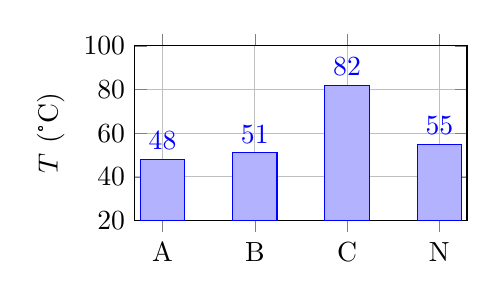
\begin{tikzpicture}
\begin{axis}[ybar,width=5.8cm,height=3.8cm,bar width=16pt,ylabel={$T$ (°C)},symbolic x coords={A,B,C,N},xtick=data,ymin=20,ymax=100,nodes near coords,grid=major]
\addplot coordinates {(A,48)(B,51)(C,82)(N,55)};
\end{axis}
\end{tikzpicture}
\end{columns}
\begin{caixaAt}
Fase C muito mais quente é um \textbf{indício}; a ação correta é diagnosticar antes de apenas ``reapertar tudo''.
\end{caixaAt}
\end{frame}

%=====================================================================
